% !TEX encoding = UTF-8 Unicode
%!TEX root = ../Main/thesis.tex
% !TEX spellcheck = en-US
%%=========================================
\documentclass[../Main/thesis.tex]{subfiles}
\begin{document}
\chapter[Fourier analysis and its application to bearing fault detection]{Fourier analysis and its application to bearing fault detection}
\label{sec:chapter2}

\section{An overview of Fourier analysis}
From solving differential equations to analyzing sound wave, images and signal in general, Fourier analysis has a profound impact in science and engineering. It provides a convenient way to transforming signals into sums of frequencies called frequency spectrum, and reveals unseen aspect of data. The bulk of Fourier analysis is to decompose a signal or more generally a function, into trigonometric extentions. 
\justify
 A signal can be viewed as a series of observations generated by a given process and recorded at discrete or continuous time interval. The underlying process might be the sum of subprocesses. In this case, the frequency domain will reveal all the subprocesses characteristics.
This is illustrated in Figure \ref{fig:fft_domain}, where a signal (in dark) is decomposed into sinusoidal components (in blue). The sinusoidal components can be represented in a coordinate system with frequencies on the x axe and amplitudes on the y axe (in red). This is called the frequency domain. From the frequency domain we can observe a hight amplitude low frequency component. As we move toward high frequencies, the amplitudes decrease.
\begin{figure}[H] %  figure placement: here, top, bottom, or page
   \centering
   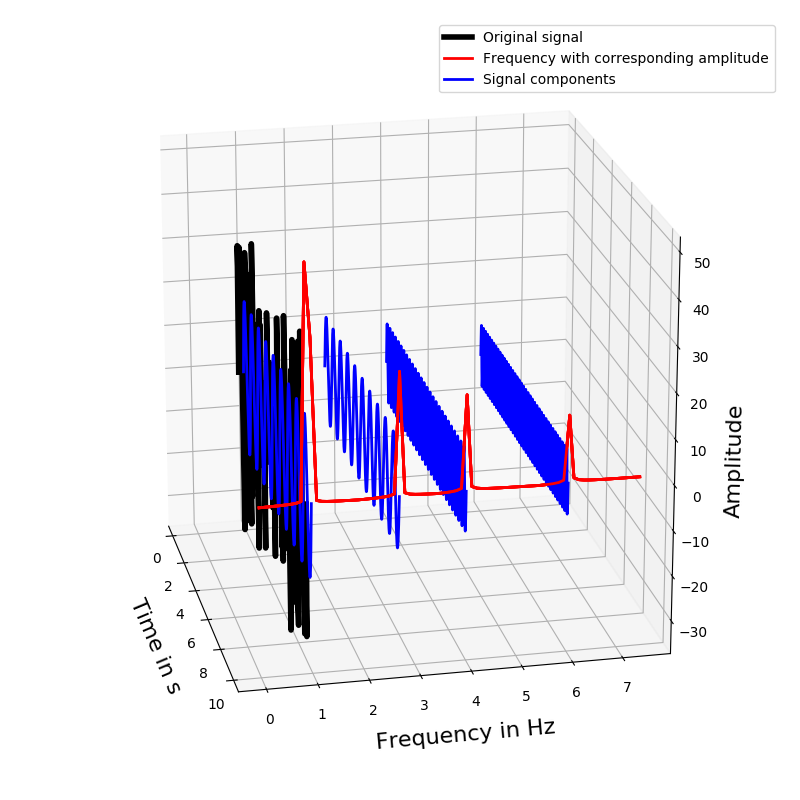
\includegraphics[width=6in]{../fig/fft_domain} 
   %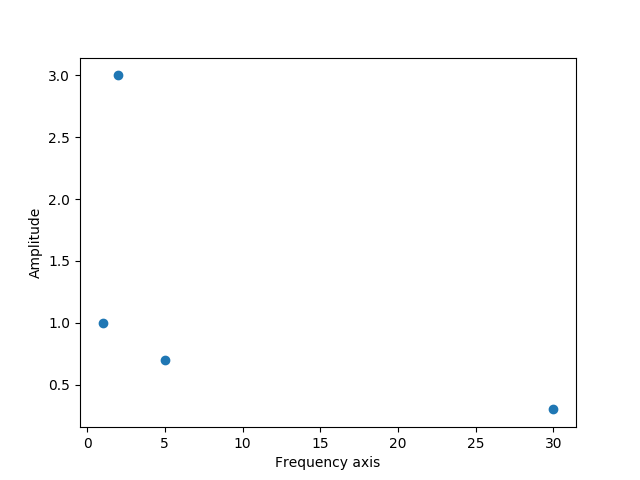
\includegraphics[width=2.5in]{freq} 
   \caption{}
   \label{fig:fft_domain}
\end{figure}
\justify
Fourier analysis is concerned with the general problem of periodic and non periodic functions approximation. The former and the latter are treated by Fourier series and Fourier transform, respectively. %Given a periodic function, its Fourier series is given as a discrete superposition of exponential functions, and its Fourier transform is given by continuous superposition of exponential functions.
%\justify
%Fourier analysis is used in a wide range of application, including signal processing, data compression, image analysis. The main objective is to take a signal or more generally a function, and decompose its in trigonometric functions. 
%%%%%%%%%%%%%%%%%%%%%%%%%%%%%%%%%%%%%%%%%%%%%%%%%%%%%%%%%%%%%

\subsection{Fourier series}
As previously mention, Fourier series is concerned with the general problem of periodic functions approximation. The basic ingredients required to approximate a function in this scenario are: a vector space, a basis, which is a subspace of the vector space, and a mathematical operation, or more generally a function such as an inner product that maps two vectors to a real number. If a vector space has an inner product, we say that the vector space is an inner product space. 
\justify
Before continuing, we see the need to clarify some abbreviations. We use the letters $f$, $V$, $V_{0}$ for an arbitrary function, a vector space, and a subspace of a vector space, respectively.
Basis functions will be denoted by $\{  \varphi_{0}, \cdots,\varphi_{n}\}$, where $n$ can either be a finite integer or infinite. Having made this clarification, let explain the concept of function approximation. 
\justify
The function approximation process in light of Fourier series goes like this: Given an arbitrary function $f$ that we seek to approximate, we pick an appropriate vector space which we call $V$, such that $f\in V$. We define a subspace $V_{0}$ of the vector space $V$ and construct an inner product on $V_{0}$, if it does not exist. Furthermore, we fine an appropriate basis of $V_{0}$.  A basis of $V_{0}$ is a set of linearly independent vectors   $\{  \varphi_{0}, \cdots,\varphi_{n}\}$ in $V_{0}$, that span $V_{0}$. 
\justify
This means that any vector in $V_{0}$ can be written as a linear combination of the basis vectors. Once we have all this in place, the best approximation of the function $f$ is its orthogonal projection in the inner product space $V_{0}$. Figure \ref{figure:il} shows an illustration of a generic mechanism of function approximation by orthogonal projection, where $f_{0}$ is the orthogonal projection of $f$ in the subspace $V_{0}$ of $V$.
\justify
\begin{figure}[H]
\begin{center}
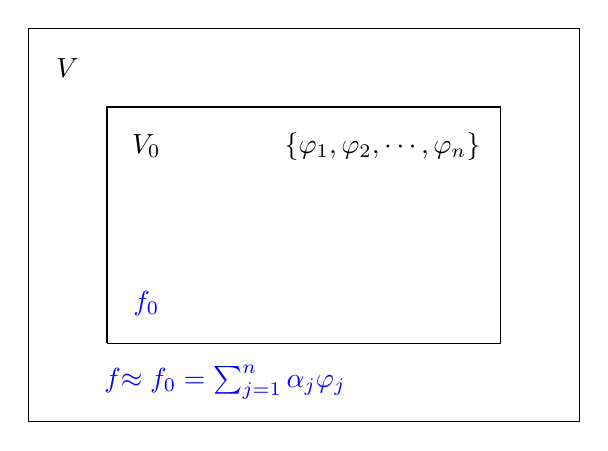
\begin{tikzpicture}
\path (0,0) coordinate (origin1);
\path(0.5,4.5) node (V){$V$};
\path(2.5,0.5) node (f){$\textcolor{blue}{f}\textcolor{blue} {\approx f_{0} = \sum_{j=1}^{n} \alpha_{j} \varphi_{j}}$};
\path (0,5) coordinate (topleft1);
\path (7,5) coordinate (topright1);
\path (7,0) coordinate (bottom1);
% draw
\draw (origin1) -- (bottom1) -- (topright1) -- (topleft1) -- (origin1);

% reactagle 2
\path (1,1) coordinate (origin2);
\path(1.5,3.5) node (V0){$V_{0}$};
\path(1.5,1.5) node (f0){$\textcolor{blue}{f_{0}}$};

\path (1,4) coordinate (topleft2);
\path (6,4) coordinate (topright2);
\path(4.5,3.5) node (b0){$ \{\varphi_{1}, \varphi_{2}, \cdots, \varphi_{n}\} $};
\path (6,1) coordinate (bottom2);
% draw
\draw (origin2) -- (bottom2) -- (topright2) -- (topleft2) -- (origin2);
\end{tikzpicture}
\end{center}
\caption{Illustration of a generic function approximation process of a function $f$ into a subspace $V_{0}$ of a vector space $V$. $\varphi_{j}$ are the basis functions and $\alpha_{j}$ are real numbers for $j=1,\cdots,n$.}
\label{figure:il}
\end{figure}

\justify
Having the generic function approximation defined in Figure \ref{figure:il} as a blue print, the Fourier space $V_{0}$ is a subspace of the space of all continuous functions of the interval $[0, T]$ and denoted by $C[0,T] $ which is $V$ in Figure \ref{figure:il}. The subspace $V_{0}$ of $V$ is spanned by 
\begin{equation}
\left\{1, \cos\left( \frac{2\pi t}{T} \right), \cdots,\cos\left( \frac{2\pi Nt}{T} \right), \sin\left( \frac{2\pi t}{T} \right), \cdots,\sin\left( \frac{2\pi Nt}{T} \right)   \right\}. \nonumber
\end{equation}
which corresponds to
\begin{equation}
\{\varphi_{1}, \varphi_{2}, \cdots, \varphi_{n}\}, \nonumber
\end{equation}
from figure \ref{figure:il}. Let $f$ be an arbitrary periodic function of period $T=2L$, defined on an interval of length $L$. Its Fourier series representation is then given by
\begin{equation}\label{eq:fs}
f_{n}(t) = \frac{a_{0}}{2} +\sum_{n=1}^{n}\left( a_{n} \cos\left( \frac{n\pi t}{L}\right) + b_{n} \sin\left( \frac{n\pi t}{L}\right)  \right), \end{equation}
where the coefficients $a_{0}, a_{1}, \cdots, b_{1}, b_{2},\cdots$, corresponding to the $\alpha_{j}$ in Figure \ref{figure:il}, are given by 
\begin{equation}\label{eq:fsc}
\begin{split}
a_{m} &= \frac{1}{L}\int_{-L}^{L}f(t)\cos\left( \frac{m\pi t}{L}\right) \mathrm{d}t,\quad m=0,1,2,\cdots\\
b_{n} &= \frac{1}{L}\int_{-L}^{L}f(t)\sin\left( \frac{n\pi t}{L}\right) \mathrm{d}t,\quad n=1,2,\cdots
\end{split}
\end{equation}
\justify
There are various condition under which the Fourier series given in (\ref{eq:fs}) converges. One such condition is the Dirichlet condition and is given by the following theorem:

\begin{theorem}
Suppose that $f$ is periodic with period $T$, and the following conditions are satisfied:
\begin{enumerate}
\item $f$ has a finite set of discontinuity in each period
\item $f$ contains a finite set of maxima and minima in each period
\item $\int_{0}^{T}|f|\mathrm{d}t <\infty$
\end{enumerate}

Then we have that 
\begin{equation}
\lim_{n\rightarrow \infty} f_{n}(t) = f(t) ,\nonumber
\end{equation}
for all t, except at those points t where f in not continuous.
\end{theorem}



%%%%%%%%%%%%%%%%%%%%%%%%%%%%%%%%%%%%%%%%%%%%%%%
\subsection{Fourier transform and the fast Fourier transform}
The Fourier series decomposes function into trigonometric extensions in $[-\pi, \pi]$, that vibrates at integer frequencies. Contrary to the Fourier series, the Fourier transform decomposes functions into extensions that vibrates at frequencies that are real number on infinite time interval [ref]. This is of great practical importance, at least for bearing fault detection, since failure failure frequencies are often real numbers.
%%%%%%%%%%%%%%%%%%%%%%%%%%%%%%%%%%%%%%%%%%%%%%%%%%%%%%%%%
\section{Application of Fourier transform for bearing fault detection: a case study}
In this section we present a case study where Fourier analysis is used to detect various bearings failure frequencies. We start by describing the experimental setup for the case study, followed by the methodology for fault detection
\subsection{Description of the case study}
The data used in this case study was generated by the Intelligence Maintenance System (IMS) [link]. Three separate experiments involving four bearings were performed on a motor. In each experiment, a one second vibration signal snapshot was recorded every five or ten minutes [reference]. Each vibration signal or what we could call sample, consists of 20 480 data points with a sampling rate of 20 000 Hz.
\justify
The sampling rate also called sampling frequency, is the average number of sample points obtained per second during the sampling process. The sampling process is the reduction of an analog signal to a digital signal. The analog signal is the continuous time signal, while the digital signal is the discrete time signal of interest.
\begin{figure}[H] %  figure placement: here, top, bottom, or page
   \centering
   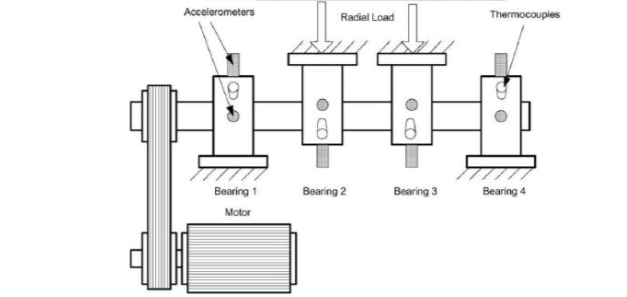
\includegraphics[width=8in]{../fig/experiment} 
   \caption{Experimental set up. [reference]}
   \label{fig:exp}
\end{figure}
\justify
Figure \ref{fig:exp} shows the experimental setup. Four bearings support a rotating shaft, driven by an AC motor through rub belts. The motor rotates at 2000 rotations per minute, while the bearings are subjected to a constant radial force of 6000 lbs [ref]. In the first experiment, height accelerometers were used, two on each bearing. One for the radial position and the other for the axial position. In the second and third experiment, four accelerometers were used, one for each bearing.
\justify
An accelerometers is a sensor that measures vibration signals. Axial signal are the signal measured by the accelerometers along the axis of the motor shaft, while radial signal are measure along the perpendicular direction of the motor shaft.
\justify
At the end of the first experiment, inner race defect occurred in bearing number 3 and roller element defect occurred in bearing number 4. At the of the second and third experiment, outer race defect occurred in bearing number 1 and number 3, respectively. In the next section we define the different types of bearing faults such as inner race defect, outer race defect and roller element defect. 
\subsection{Bearing faults}
As pointed out earlier, the bearing failure frequencies depends on the geometry of the bearing and the rotating speed of the motor. Figure \ref{fig:bearing} shows a blow up view of a bearing. In the figure we see the outer ring of the bearing (1), the cage (3) which holds the cylindrical rolling elements (2) and the inner race (4 and 5).
\begin{figure}[H] %  figure placement: here, top, bottom, or page
   \centering
   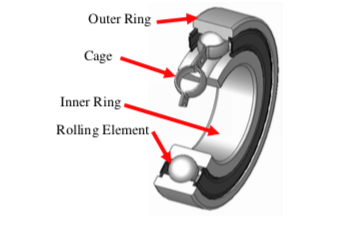
\includegraphics[width=3.2in]{../fig/bearing} 
    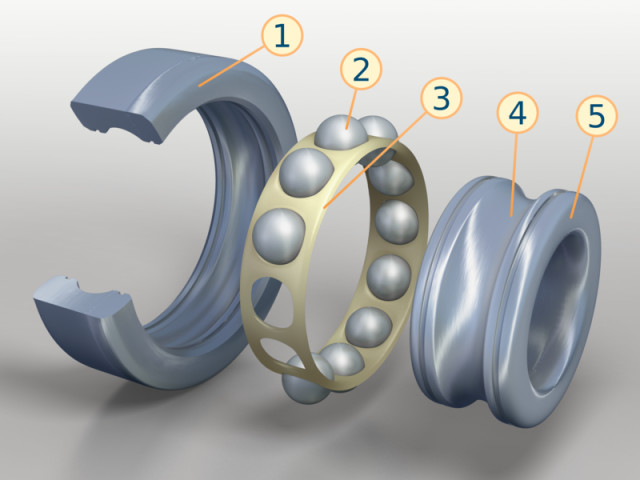
\includegraphics[width=3.2in]{../fig/bearing-s} 
   \caption{Geometrical description of a bearing left(ref), right(ref)}
   \label{fig:bearing}
\end{figure}
\justify
Inner race defect and outer race defect are defect occurring at the inner race and outer race, while roller element defect also called ball spin happens when a roller element is defectuous. Any of the defect occurs at a specific frequency that can be computed based on the bearing geometry and the rotation speed of the machine. inner race defect occurs at a frequency called ball pass frequency inner race (BPFI), outer race defect occurs at a frequency call ball pass outer frequency outer race (BPFO) and roller element defect occurs at a frequency call ball spin frequency (BSF). They are expressed in Hz in terms of the bearing geometry as 
\begin{equation}\label{eq:bpfi}
BPFI = \frac{nb}{2}S\left( 1 +  \frac{BD}{PD}\cos(\beta)  \right)
\end{equation}

\begin{equation}\label{eq:bpfo}
BPFO = \frac{nb}{2}S\left( 1 -  \frac{BD}{PD}\cos(\beta)  \right)
\end{equation}

\begin{equation}\label{eq:bpfi}
BSF = \frac{PD}{2BD}S\left( 1 -  \left(\frac{BD}{PD}\cos(\beta)\right)^{2}  \right)
\end{equation}
\clearpage
where 
\begin{itemize}
\item S is the rotating speed of the motor
\item nb is the number of cylindrical balls (roller elements)
\item BP is the the ball diameter
\item PD is the pitch diameter
\item $\beta$ is the contact angle
\end{itemize}
The pitch diameter is the perpendicular distance from the center of one ball to the center of the ball located at the end. The contact angle can be taken to be zero?
\subsection{Failure detection methodology}
Given a vibration signal measured from an accelerometer, our intent is to detect the presence of a forcing frequency. By forcing frequency we refer to either BPFO, BPFI or BSF. Recall that a forcing frequency is a fancy name for failure frequency. We will refer to the vibration signal as the time domain signal, as it is customary to do so. Since the forcing frequencies are in Hz, the time domain signal must be transformed into frequency domain signal. The frequency domain signal is also called the frequency spectrum. The reader can refer to Figure \ref{fig:fft_domain} for a reminder. Once we have the frequency spectrum corresponding to the original time signal, we can look for the presence of any forcing frequency.
\justify
There are four steps in transforming time domain signal into frequency domain signal: A band pass filtering, enveloping, a low pass filtering and a fast Fourier transformation.
Figure \ref{fig:fft-process} shows a schematic description of the entire process. Let elaborate on it.  A vibration signal from a bearing accelerometer contains not only the vibration signal of the bearing, but also the signal from other components, such as motor, shaft and so on.
\justify
The band pass filter allows signal within a given band of frequency to seep through, while attenuating all other signal. The band of allowed frequencies is bounded bellow and above by two parameters: The low cut-off frequency and the high cut-off frequency, respectively.
%The intent is to only capture bearing vibration signal and ignore any other. Once this done, the demodulation extract the high frequency time domain signal and a low pass filter extract the low frequency. The Fast Fourier transform is then applied to the time domain signal to generate the frequency spectrum.
\begin{figure}[H]
\begin{tikzpicture}
  [node distance=.8cm,
  start chain=going below,]
     \node[punktchain, join] (intro) {Signal};
     \node[punktchain, join] (probf)      {Band pass filtering};
     \node[punktchain, join] (investeringer)      {Enveloping};
     \node[punktchain, join] (perfekt) {Low pass filtering};
     \node[punktchain, join, ] (emperi) {Fast Fourier transform};
     % \node (asym) [punktchain ]  {Asymmetrisk information};
      \begin{scope}[start branch=venstre,
        %We need to redefine the join-style to have the -> turn out right
        every join/.style={->, thick, shorten <=1pt}, ]
        \node[punktchain, on chain=going left, join=by {->}] (risiko) {Frequency spectrum};
      \end{scope}
      \begin{scope}[start branch=hoejre,]
      %\node (finans) [punktchain, on chain=going right] {Det finansielle system};
    \end{scope}
    \end{tikzpicture}
  \caption{Process of obtaining a frequency spectrum from an input signal}
   \label{fig:fft-process}
\end{figure}
\justify
The enveloping step corresponds to rectifying the signal by accounting only for the positive part of the signal. Let $E(t)$ be the signal resulting from the enveloping process. Let $x(t)$ is the time domain signal, and let its Hilbert transform be denoted by $H(t)$. Then we have
\begin{equation}
H(t) = \frac{1}{\pi}P\int_{-\infty}^{+\infty}\frac{x(t)}{t-\tau}\mathrm{d}\tau
\end{equation}
\begin{equation}
E(t) = \sqrt{H(t)^{2}+ x(t)^{2}}
\end{equation}
where $P$ is the Cauchy principal value. After the enveloping process, the resulting signal is filtered by removing hight frequency noise and the fast Fourier transform is applied to obtain the frequency spectrum.
\clearpage
\subsection{Simulation results from the experiment}
In this section we present the results resulting from applying Fourier analysis to detecting two types of faults in bearing, namely: ball pass frequency outer race defect (BPFO) and ball pass frequency inner race defect (BPFI). Recall that BPFO occurs when a defect is initiated in the outer ring of the bearing and BPFI is the defect that is initiated in the inner ring of the bearing. The reader can refer to Figure \ref{fig:bearing} for a detailed geometry description of a bearing. The experimental setup for the bearings are given in Figure \ref{fig:exp}. The bearing used in these experiments are manufactured by the company Rexnord, and are of type Rexnord ZA 2115, with forcing frequencies  given by 
\begin{equation}
BPFO = 236.4 Hz, \quad BPFI = 296.8 Hz \nonumber
\end{equation}
We apply the process described in Figure \ref{fig:fft-process} for experiment 1, 2 and 3
\subsubsection{Result for experiment 2}
In experiment number 2, successive vibration samples where measured from bearing number 1,2,3 and 4, resulting in 984 samples for each bearing.  At the end of the experiment, BPFO defect occurs in bearing number 1. Figure \ref{fig:bearing1-experiment2} shows the vibration signal from sample number 900, measured from bearing number 1. Figure \ref{fig:bearing1-experiment2-fft} shows the corresponding frequency spectrum obtained by applying the process described in Figure \ref{fig:fft-process}.
\justify
In the frequency spectrum, we can clearly identify the BPFO frequency (in orange), which has the largest amplitude in the spectrum. We can also observe three harmonics of the BPFO.
BPFO harmonics are multiple frequency of the BPFO frequency. Here we observe $2\times$BPFO, $3\times$BPFO and $4\times$BPFO harmonics. The BPFO frequency are characterized by the presence of harmonics [ref:Vib analy training manuel cat1]. 
\justify
In contrast to Figure \ref{fig:bearing1-experiment2-fft}, Figure \ref{fig:bearing2-experiment2-fft}, \ref{fig:bearing3-experiment2-fft} and \ref{fig:bearing4-experiment2-fft}, show respectively the frequency spectrum of bearing number 2,3 and 4. These spectrum can been seen as noise compare to the spectrum of bearing number 1, which suffers from BPFO defect. It is worth noting that the BPFO defect usually appears at the bottom of the bearing where the load experienced by the bearing is the largest.
\begin{figure}[H] %  figure placement: here, top, bottom, or page
   \centering
   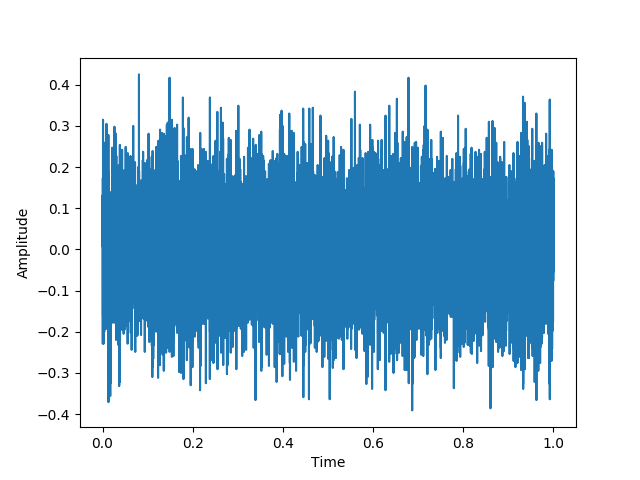
\includegraphics[width=6in]{../fig/experiment2_bearing1.png} 
   \caption{Vibration signal corresponding to sample 900, from bearing number 1 in  experiment 2}
   \label{fig:bearing1-experiment2}
\end{figure}
%%%%%%%%%%%%%
\begin{figure}[H] 
   \centering
   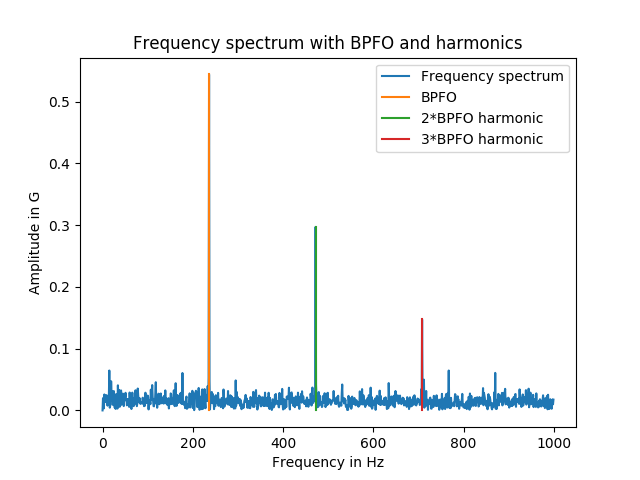
\includegraphics[width=6in]{../fig/experiment2_bearing1_fft.png} 
   \caption{Frequency spectrum obtained from vibration signal corresponding to sample 900, of bearing number 1,  in  experiment 2}
   \label{fig:bearing1-experiment2-fft}
\end{figure}

\begin{figure}[H] 
   \centering
   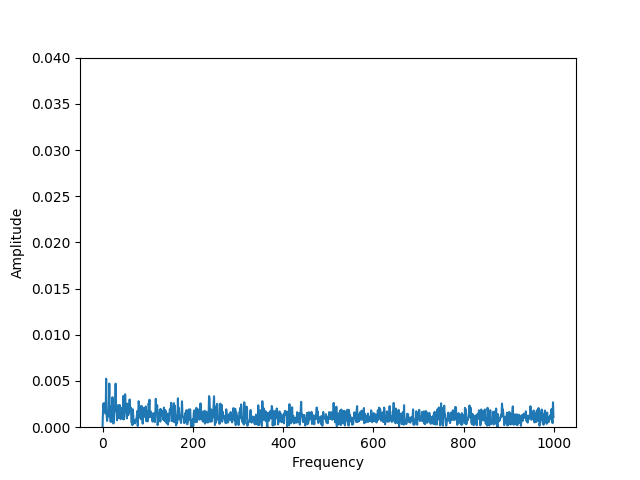
\includegraphics[width=6in]{../fig/experiment2_bearing2_fft.png} 
   \caption{Frequency spectrum obtained from vibration signal corresponding to sample 900, of bearing number 2, in experiment 2.}
   \label{fig:bearing2-experiment2-fft}
\end{figure}

\begin{figure}[H] 
   \centering
   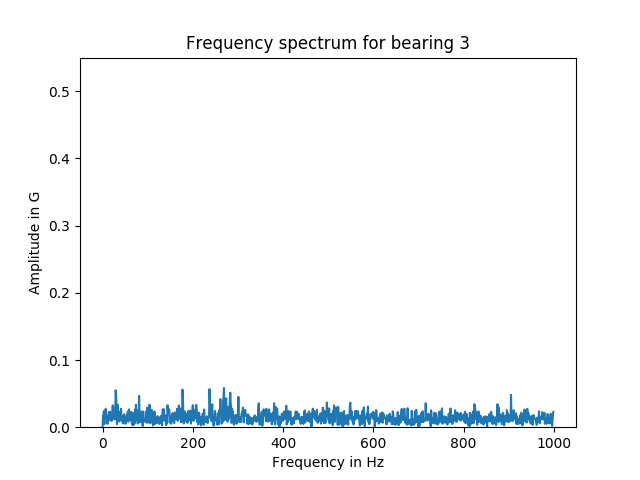
\includegraphics[width=6in]{../fig/experiment2_bearing3_fft.png} 
   \caption{Frequency spectrum obtained from vibration signal corresponding to sample 900, of bearing number 3, in experiment 2.}
   \label{fig:bearing3-experiment2-fft}
\end{figure}

\begin{figure}[H] 
   \centering
   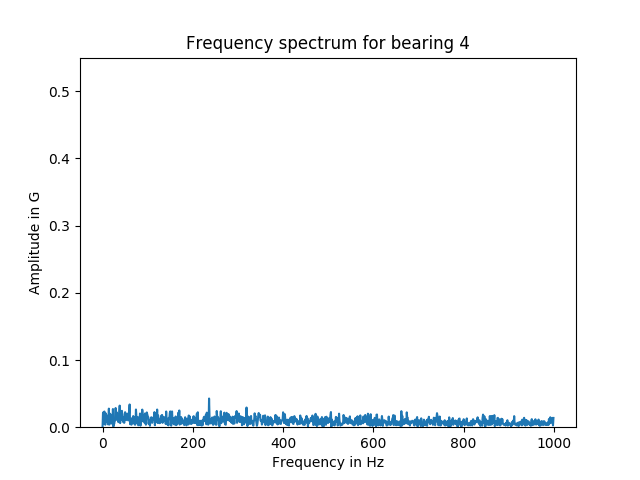
\includegraphics[width=6in]{../fig/experiment2_bearing4_fft.png} 
   \caption{Frequency spectrum obtained from vibration signal corresponding to sample 900, of bearing number 4, in experiment 2.}
   \label{fig:bearing4-experiment2-fft}
\end{figure}
\justify
Now let compare all bearing. To do so we compute the BPFO frequency, and related amplitude for each sample. Figure \ref{fig:experiment2_bearing_fft_trend} shows 
the trend of the BPFO amplitude as the experiment evolve. We can observe that at the beginning of the experiment, bearing number 1 had a significant large failure amplitude.
As the experiment evolve, the amplitude increases almost steadily, until failure occurs. In contrast to bearing 1, bearing 2, 3 and 4 BPFO amplitude are relatively steady during the experiment. 
\begin{figure}[H] 
   \centering
   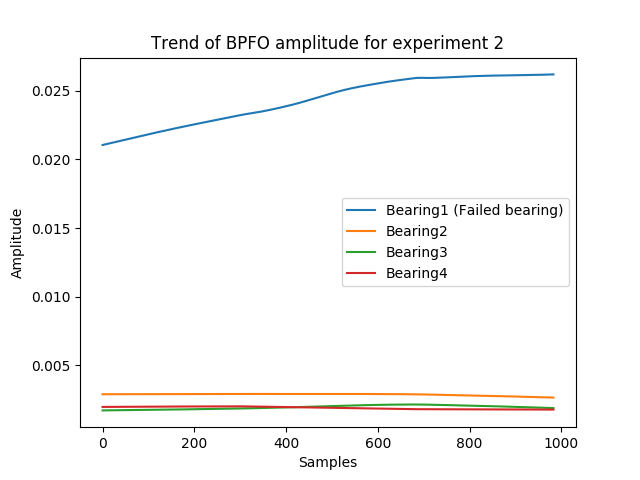
\includegraphics[width=6in]{../fig/experiment2_bearing_fft_trend.png} 
   \caption{Trend for BPFO for each samples}
   \label{fig:experiment2_bearing_fft_trend}
\end{figure}

\justify
\subsubsection{Experiment 1 and 3}
























\blankpage
\end{document}

